\title{Project 1: Navigation}
\author{
	Rory McGrath \\
}
\date{\today}

\documentclass[12pt]{article}
\usepackage[margin=1in]{geometry}
\usepackage{graphicx}

\begin{document}
\maketitle

\section{Overview}
For this project an agent was trained to navigate a large square world and collect bananas.
A reward of +1 was provided for collecting a yellow banana, and a reward of -1 was provided for collecting a blue banana.
The goal of the agent is to collect as many yellow bananas as possible within a given timeframe while avoiding blue bananas.

For this project the state space has 37 dimensions. These attributes represented the agent's velocity along with the ray-based perception
of objects around the agent's forward direction.
The action was able to perform 4 distance actions:

\begin{itemize}
\item 0 - move forward
\item 1 - move backward
\item 2 - turn left
\item 3 - turn right
\end{itemize}

The given task to solve is episodic. 
A agent is said to have 'solved' the environment if it can achieve a score of +13 over 100 consecutive episodes.

\section{Proposed Methods}
\label{methods}
In order to solve this environment Deep Q-Networks \ref{deep_q_networks} were implemented.
In general, Deep Q-Networks are used as a functional approximation  when estimating the optimal action-value function $Q_*$.
Instead of performing a table lookup, which does not scale well with the action space and state space, a neural network is trained
on past experiences to estimate the action-value function for the current state and actions.

One of the main issues when initially using a neural network to estimate an optimal action-value function 
is how to you obtain the targets for back-propagation?
The answer is relatively straight forward.
Firstly we assume we are solving the environment using temporal difference (TD) and are provided with the data in 
the SARSA format, (state, action, reward, next\_state, next\_action) denoted by (s, a, r, s', a').

\begin{enumerate}
	\item Firstly we estimate the Q value of s' using forward propagation.
	\item Next we calculate the Q value for the current state s by substituting the estimated next state values Q(s',a') 
			into the equation:
	\begin{center}
		$q(s,a) = r+\gamma Q(s',a') $
	\end{center}
	\item We then estimate the value of q(s, a) denoted by \^q(s, a) using forward propagation of our ANN.
	\item Finally our ANN is then trained via back propagation using  \^q(s, a) as our prediction and our calculated q(s, a) as the target.
\end{enumerate}

Although this may seem confusing to update our estimate with an estimate, by introducing the actual observed reward r 
and assuming sufficient exploration of the state space the Q values will tend towards their actual values.

Their are, however, two main issues with this naive approach. 
Firstly, as we view (s, a, r, s', a) tuples as they are created, 
given the nature of the environment they can be highly correlated.
This can cause action values to oscillate or diverge catastrophically.
Secondly, since we are updating a guess with a guess this can lead to harmful correlations if we updated the ANN weights on each time step.
To combat these issues Experience Replay\ref{experience_replay} and Fixed Q-Targets\ref{fixed_q_targets} were implemented.

\section{Results}

Using the methodology described above [\ref{methods}] an agent was trained to solve the environment.
The agent was written in pyTorch and was run using the openai gym toolkit.

The ANN used for the agent consisted of an input layer of 37 nodes, one dense hidden layer of 148 nodes and an output layer of 4 nodes.
All activation functions were rectified linear units (ReLUs). 
As we are not dealing with probabilities a softmax function on the output layer was not required.

The following hyper-parameters were used to train the model:


\begin{table}[h!]
\begin{center}
\begin{tabular}{|l|l|}
	\hline
	\multicolumn{2}{|c|}{\textbf{Learning Updates}}\\
	\hline
	\textbf{Parameter} & \textbf{Value}\\
	\hline
	$\gamma$ & $0.99$\\
	$\alpha$ & $5e^{-4}$\\
	$\epsilon$ & 1.0 to 0.01 with a rate of decay of 0.995 per episode\\
	\hline
\end{tabular}
\end{center}
\end{table}

\begin{table}[h!]
\begin{minipage}{.5\linewidth}
\begin{tabular}{|l|l|}
	\hline
	\multicolumn{2}{|c|}{\textbf{Experience Replay}}\\
	\hline
	\textbf{Parameter} & \textbf{Value}\\
	\hline
	Buffer Size & $1e^{5}$\\
	Batch Size & $64$\\
	\hline
\end{tabular}
\end{minipage}
\begin{minipage}{.5\linewidth}
\begin{tabular}{|l|l|}
	\hline
	\multicolumn{2}{|c|}{\textbf{Fixed Q}}\\
	\hline
	\textbf{Parameter} & \textbf{Value}\\
	\hline
		$\tau$ & $1e^{-3}$\\
		Update Rate & every 4 time-steps \\
	\hline
\end{tabular}
\end{minipage}
\end{table}

The model was trained for 1500 episodes. 
After 1200 episodes the model achieved it's target of an average of +13 over 100 episodes.
A plot of the reward verses episode number is given in [Fig \ref{results}].

\begin{figure}
	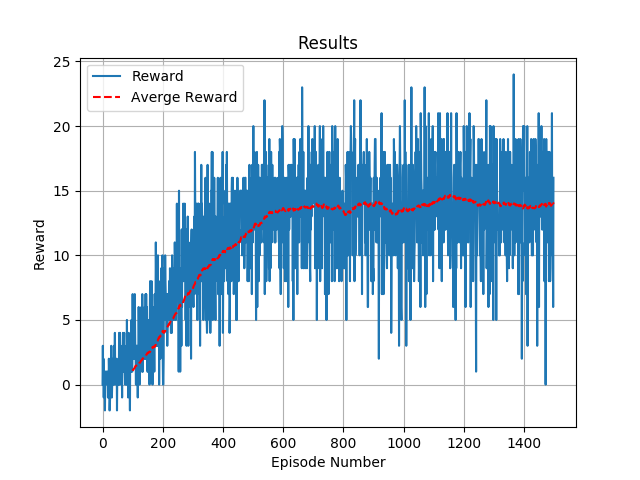
\includegraphics[width=\linewidth]{./img/Results.png}
	\caption{Training results}
	\label{results}
\end{figure}

\section{Future Work}
While the initial results of this agent are promising, the agents behaviour is far from optimal.
There are several improvements that could be implemented to decrease training time and increase the average reward.

A hyper-parameter optimisation technique such as grid search could be implemented to help converge on good choices of the parameters 
specified above. Ideally this would be run on a gpu server.

The Replay Buffer could be updated to implement prioritised experience replay \ref{per_paper}. 
The key idea here is that 'important' transitions would be sampled more frequently than unimportant ones. 
The 'important' of transition is determined by the magnitude of it's temporal-difference error.
This should allow the agent to learn more efficiently. 
Given that we are no longer uniformly sampling from the experiences importance sampling will have to be added to calculate the impact of each weight when updating.

The agents learning method could be updated to implement Double DQN \ref{ddqn_paper}. 
Currently in the agent uses the same value to select and action and then evaluate that action.
This can lead to over optimistic value estimates.
To overcome this the action selection can be decoupled from the evaluation.
In the case of our implementation we can partially decoupling the action selection and evaluation by selection the action using the local q network and evaluating the action on the target Q network.
\end{document}
